\section{ArquitecturaGeneral}
\label{sec:ArquitecturaGeneral}

El desarrollo de las pruebas de este proyecto se realiza através de tres plataformas; la de simulación, la de entrenamiento del modelo y la de inferencia. En este apartado se explican estas de manera general, para crear una base de entendimiento del pipeline. En los proximos apartados del capitulo se explica cada elemento de manera más exhaustiva, con las distintas iteraciónes y mejoras conseguidas a raíz de la investigación.

\begin{figure}[H]
	\centering
	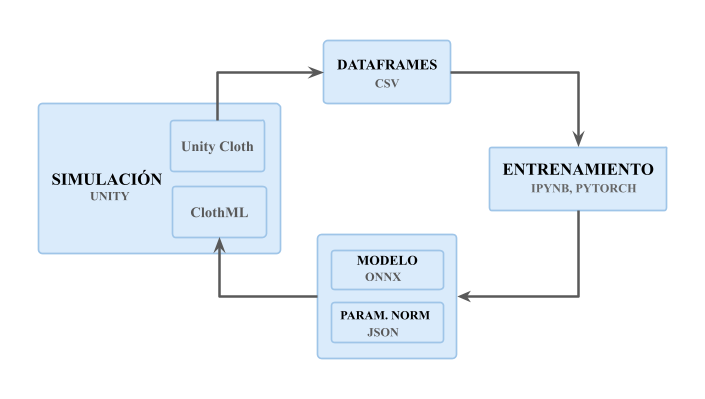
\includegraphics[width=1\textwidth]{Imagenes/Arquitectura.png}
	\caption{Diagrama de la arquitectura General del proyecto}
\end{figure}

Como puede apreciarse en la figura, el pipeline del proyecto es circular, es decir, la plataforma en la que se genera la simulación y posteriormente se prueba al inferencia del modelo es la misma, en nuestro caso Unity. Esto se debe a dos de nuestros objetivos, el de hacer un sistema accesible y fácil de utilizar y el de poder comparar verazmente la optimización de la simulación física. \newline

Si bien se han llevado a cabo puebas con distintas geometrias y tiempos, colisionadores con distintos tipos de movimiento y aleatoriedad de los mismos, las base de las escenas es equivalente. La simulación, en nuestro caso creada con el sistema de Cloth de Unity, pasa por un sistema de registro con el que se crea un archivo CSV que recoge la información de la geometría simulada y las variables pertinentes. Estos archivos se recogen en una carpeta que pasa a procesarse en un entorno de python. Con las librerias explicadas en el estado del arte, se han entrenado distintos modelos, iterando sobre ellos para conseguir las configuraciones e hiperparámetros más optimos. La efectividad de estos modelos se mide en primer lugar con el "accuracy" de las predicciones, visualizando la progresión de las predicciónes atraves de distintos frames y etc. Posteriormente se exportan estos modelos ya entrenados en formato ONNX a la escena de Unity en la que se hizo la recogidad de datos. Hanciendo uso de la arquitectura dirigida a objetos de Unity, se cambia la configuración de la geometría inicial y se incorpora el modelo entrenado y sus parámeteros, consiguiendo así inferir el movimiento de la tela en tiempo real y confirmar que la simulación es visualmente fiel a las físicas reales. \newline